\documentclass[a4paper,11pt]{article}

%\usepackage{ctex}

%tables, figures, lists, citation
\usepackage{float}
\usepackage{booktabs}
\usepackage{multirow}
\usepackage{graphicx}
\usepackage{subfigure}
\usepackage{enumitem}
\usepackage{mdwlist}
\usepackage{cite}
\usepackage{url}
\usepackage{authblk}
\makeatletter
\def\@cite#1#2{\textsuperscript{[{#1\if@tempswa , #2\fi}]}}
\makeatother

%math
%style mathematica
%special fonts, hollow fonts
%\mathds{A} \mathbb{1} \mathbbm{i}
\usepackage{dsfont, mathbbol, bbm, mathrsfs}
\usepackage{amsmath, amssymb, mathrsfs, bm}
\newcommand{\mathee}{\mathbbm{e}}
\newcommand{\mathii}{\mathbbm{i}}
\newcommand{\mathdd}{\mathrm{d}}

%geometry
\usepackage{geometry}
\geometry{left=1.7cm,right=1.7cm,top=1.9cm,bottom=1.6cm}

%usage of \astrosun
\usepackage{wasysym}

%numberwithin
\numberwithin{equation}{section}
\numberwithin{table}{section}
\numberwithin{figure}{section}



\begin{document}
	
	
	\title{On the Equilibrium of White Dwarfs}
	\author{Yiqi Xie\thanks{Student ID: 1300011383. Email: xieyiqi@pku.edu.cn}}
	\affil{\textit{School of Physics, Peking University}}
	\date{July 6, 2017}
	\maketitle
	\thispagestyle{empty}
	\begin{abstract}
		A model for non-rotating spherical helium white dwarfs was built and its equilibrium was solved. Electron degenerate pressure and Newtonian gravitational field were taken into consideration, based on which a key equation on the distribution of electron chemical potential was derived. We first checked the equation at the non-relativistic limit and the ultra-relativistic limit, then a general solution was obtained through numerical methods determined with adequate deliberation. We also calculated the density distribution and the total mass for a spectrum of white dwarfs, from which the contribution of relativistic effect to the complete collapse of the star was illustrated. The upper mass limit for a white dwarf to stand such collapse, namely the Chandrasekhar limit, has been derived as $1.44M_{\astrosun}$ in this paper, which is consistent with the number formerly provided by Chandrasekhar himself.
	\end{abstract}
	
	\section{Introduction}
	
		White dwarfs, in observation, are abnormally faint for their color\cite{schatzman1958whitedwarfs}. They are the core remnants, the final evolutionary stage, of stars whose mass is at a low or medium level\cite{richmond2007latestages}. A typical white dwarf is composed mostly of helium\cite{pathria2012statmech}, the product of hydrogen fusion reaction happened in its former evolutionary stages, and for some cases, heavier elements such as carbon and oxygen might also be found. Unable to fuse these elements by itself, a white dwarf cannot generate enough thermal pressure in against of gravity, and as a result, it collapses into a highly compressed state. The mass of a typical white dwarf is comparable to that of Sun, while its volume is comparable to that of Earth\cite{williams2013sunfact}\cite{johnson2007extreme}. Under such high density, the electron degeneracy pressure arises in place of thermal pressure\cite{fowler1926dense}, so that the star stablizes at a new equilibrium. Here we list some chararistic physical properties of a white dwarf in contrast with the Sun in Table \ref{tab:phyprop}.
		\begin{table}[ht]
			\centering
			\caption{White Dwarf Sketch\cite{williams2013sunfact}\cite{johnson2007extreme}}
			\begin{tabular}{r@{ }c@{}lcc}
				\toprule
				\multicolumn{3}{c}{~~Parameter} & White Dwarf & Sun (in Contrast) \\
				\midrule
				Mass & $M$ & $/~\!\mathrm{g}$ & $\sim 10^{33}$ & $\sim 10^{33}$ \\
				Radius & $R$ & $/~\!\mathrm{cm}$ & $\sim 10^{9\phantom{1}}$ & $\sim 10^{11}$ \\
				Density & $\rho$ & $/~\!\mathrm{g\cdot cm^{-3}}$ & $\sim 10^{6\phantom{1}}$ & $\sim 10^{0\phantom{1}}$ \\
				Temperature & $T$ & $/~\!\mathrm{K}$ & $\sim 10^{7\phantom{1}}$ & $\sim 10^{7\phantom{1}}$ \\
				\bottomrule
			\end{tabular}%
			\label{tab:phyprop}%
		\end{table}
	
		As mentioned above, the equilibrium between degenerate pressure and gravitational force holds the white dwarf in its shape. From such equilibrium it is possible to derive the constraints for a white dwarf's mass, radius, etc. Exact work has been done by Chandrasekhar in 1931-1935\cite{chandrasekhar1935highly}\cite{chandrasekhar1931highly}, where he stressed that the influence of relativistic effect in leading a white dwarf to collapse completely as its mass reaching to a limit - later been named after him - of $1.44M_{\astrosun}$. In following sections of this paper we will reformulate this work from our own perspective and see if we can derive Chandrasekhar's exact result.
		
		
		
	\section{Modeling a White Dwarf}
	
		\subsection{Thermaldynamics for Degenerate Electrons}
			\label{sct:intro-electron}
			
			For the beginning let us discuss a little further on the degenerate electrons of white dwarf matters. To make it simple, we neglect the electron-electron interaction and the electron-nuclei interaction, so that the system of electrons could be treated as ideal gas - it is quite a proper model since we are dealing with matter at $\sim10^7\mathrm{K}$ where everything gets highly ionized. 
			
			According to quantum field theory, electron is a fermion that obeys the Pauli exclusion principle. When highly compressed in space, electrons, by intuition, have to distinguish each other in their momentum, thus even at the temperature of absolute zero, most electrons are still fastly moving around, resulting in a non-zero pressure, namely the degeneracy pressure.
			
			Degenerate electron gas at finite temperature experiences both ordinary thermal pressure and degeneracy pressure. However, when the temperature is not too high, degeneracy pressure still steadily dominates\cite{pathria2012statmech}. In a more specific way, the above condition for temperature writes
			\begin{align}
				k_BT\ll\epsilon_F, 
				\label{eqn:TF_condition}
			\end{align}
			where $\epsilon_F$, or Fermi energy, represents the chemical potential of the electron gas at $T=0$. The value of $\epsilon_F$ can be calculated from the number density $n$ of the gas by 
			\begin{align}
				\epsilon_F=\sqrt{p_F^2c^2+m_e^2c^4}-m_ec^2, \quad
				p_F=(3\pi^2n)^{1/3}\hbar.
				\label{eqn:ef-n}
			\end{align}
			Note that for safety we have applied relativistic dispersion relation in (\ref{eqn:ef-n}), where $p_F$ is the momentum corresponding to $\epsilon_F$. Since we are dealing with white dwarfs made of helium, that every electron is bonded with one proton plus one neutron, we may substitute number density $n$ by mass density $\rho$ through
			\begin{align}
				n\approx\frac{\rho}{2m_p}.
				\label{eqn:n-rho}
			\end{align}
			Recall the information in Table \ref{tab:phyprop}, we take $\rho\sim10^6\mathrm{g\cdot cm^{-3}}$, and by (\ref{eqn:ef-n}) and (\ref{eqn:n-rho}) the calculation will give $\epsilon_F\sim10^5\mathrm{eV}$. On the other hand we see $k_BT\sim10^3\mathrm{eV}$, so that the condition in (\ref{eqn:TF_condition}) is well satisfied. Therefore, when dealing with the thermaldynamics of degenerate electron gas of a white dwarf, one may take $T=0$ and consider degeneracy pressure as the only mechanism against gravity. In addition, it is important to note that $\epsilon_F$ is comparable to the rest energy of an electron, so we shall conclude that the application of relativistic dispersion relation in (\ref{eqn:ef-n}) is necessary.
			
			Till now we haven't inspected any specific behavior of degeneracy pressure yet - actually we do not need to know many details except for its relation to density or to Fermi energy. Recall Gibbs-Duhem equation: 
			\begin{align}
				N\mathdd\mu=-S\mathdd T+V\mathdd P.
			\end{align}
			With $T$ been considered zero in our case, the $\mathdd T$ term get crossed out, reducing the equation to
			\begin{align}
				n\mathdd\mu=\mathdd P,
				\label{eqn:mu-P}
			\end{align}
			where for now $\mu$ is the same of $\epsilon_F$ and $P$ stands totally for the degeneracy pressure. We will see that (\ref{eqn:mu-P}) is good enough for later discussion.
			
		\subsection{Equation of Equilibrium}
		
			We consider only non-rotating white dwarfs, where centrifugal force does not exist. Non-rotating white dwarfs basically live on an equilibrium merely between the electron degeneracy pressure and the gravitational force. Witnessed the special relativistic nature of the densed electron gas, one may also be cautious on the general relativistic effect of the gravity. Luckily such effect is negletable, for the escape velocity of a typical white dwarf - roughly estimated as the order of $\sqrt{GM/R}\sim 10^8\mathrm{cm\cdot s^{-1}}$ - is still much lower than the speed of light\cite{schultz2009GR}. Thus we consider that the form of Newtonian gravitational field is fairly acceptable, and the equation of equilibrium writes
			\begin{align}
				\nabla P+\rho\nabla\phi=0, \quad
				\nabla^2\phi=4\pi G\rho.
				\label{eqn:P-phi}
			\end{align}
			In formar section we have clarified the relations between $\mu$, $P$ and $\rho$. Putting (\ref{eqn:ef-n}), (\ref{eqn:n-rho}) and (\ref{eqn:mu-P}) together with (\ref{eqn:P-phi}), reducing for several steps, and taking spherical symmetry, we can now express the equation of equilibrium in the spatial distribution of $\mu$: 
			\begin{align}
				\frac{1}{r^2}\frac{\mathdd}{\mathdd r}
					\left(r^2\frac{\mathdd\mu}{\mathdd r}\right)
					+\frac{16Gm_p^2}{3\pi\hbar^3c^3}
					\cdot\mu^{3/2}(\mu+2m_ec^2)^{3/2}=0.
				\label{eqn:mu_eq}
			\end{align}
			where $r$ represents the radial distance. 
			
			We consider (\ref{eqn:mu_eq}) as the key equation to solve in this paper. Categorically it is a second order differential equation wanting two boundary conditions to define its solution, one of which should apparently be that density decreases to zero on the surface, and the other of which comes from the requirement of symmetry that the gradient of any distributed physical parameter should converge to zero at the center. So we add
			\begin{align}
				\mu\bigg|_{r=R}=0,\quad
				\frac{\mathdd\mu}{\mathdd r}\bigg|_{r=0}=0.
				\label{eqn:mu_bd}
			\end{align}
			Once we solved $\mu(r)$, the distribution of density can be easily derived through
			\begin{align}
				\rho=\frac{2m_p}{3\pi^2\hbar^3c^3}\cdot
					\mu^{3/2}(\mu+2m_ec^2)^{3/2},
				\label{eqn:rho-r}
			\end{align}
			as a result from (\ref{eqn:ef-n}) and (\ref{eqn:n-rho}), and by integral a constraint on $M$ and $R$ arises as
			\begin{align}
				M=\int_0^R\!\!4\pi\rho r^2\mathdd r
					=-\frac{R^2}{2Gm_p}\frac{\mathdd\mu}{\mathdd r}\bigg|_{r=R}.
				\label{eqn:M-R}
			\end{align}
			Now we have completed a model for non-rotating spherical helium white dwarfs and derived the equation of equilibrium as specific as possible. For the following sections we will move on to the solution of (\ref{eqn:mu_eq})-(\ref{eqn:M-R}). Here we construct three constants as below that will later be frequently used:
			\begin{align}
				\left\{\begin{aligned}
					R_0&=\left(\frac{3\pi\hbar^3}{64Gm_p^2m_e^2c}\right)^{1/2}
						\approx 1.93\times 10^8\mathrm{cm} \\
					M_0&=\left(\frac{3\pi\hbar^3c^3}{64G^3m_p^4}\right)^{1/2}
						\approx 1.42\times 10^{33}\mathrm{g} \\
					\rho_0&=\frac{16m_pm_e^3c^3}{\pi^2\hbar^3}
						\approx 4.71\times 10^7\mathrm{g\cdot cm^{-3}}
				\end{aligned}\right. .
				\label{eqn:consts}
			\end{align}
			We may note that all these constans are characteristic for a typical white dwarf.
	
	
	\section{Solution to the Equation of State}
	
		\subsection{Preliminary Analysis}
			For tentative treatment, we take noramlization
			\begin{align}
				\xi=\frac{r}{R},\quad f=\frac{\mu}{2m_ec^2}.
			\end{align}
			As a result, (\ref{eqn:mu_eq}) with (\ref{eqn:mu_bd}) turns into
			\begin{align}
				\left\{\begin{gathered}
					\frac{1}{\xi^2}\frac{\mathdd}{\mathdd\xi}
						\left(\xi^2\frac{\mathdd f}{\mathdd\xi}\right)
						+\left(\frac{R}{R_0}\right)^2f^{3/2}(f+1)^{3/2}=0 \\
					f\bigg|_{\xi=1}=0,\quad
						\frac{\mathdd f}{\mathdd\xi}\bigg|_{\xi=0}=0
				\end{gathered}\right. .
				\label{eqn:rel_f}
			\end{align}
			From the first sight we realize that this is a indefinite equation with one variable parameter $R$. Since the only restriction on $R$ is positivity, our equation is doomed to suffer from numerical deformation when $R$ varies over the full range of $(0,+\infty)$. Such deformation would cause difficulties in solution, and for some cases we have to adjust our normalization on $\mu$. More specifically: 
			\begin{itemize}
				\item For $R/R_0\sim 1$: this is the only good case for (\ref{eqn:rel_f}), where $f\sim 1$ and the relativistic nature of the electron gas remains authentic;
				\item For $R/R_0\gg 1$: this is where $f$ has to be very small in order to balance the equation, and the electron gas reaches the non-relativistic end. Better choice of normalization on $\mu$ might be $f_n=(R/R_0)^4\cdot f$, so that (\ref{eqn:rel_f}) becomes
				\begin{align}
					\left\{\begin{gathered}
						\frac{1}{\xi^2}\frac{\mathdd}{\mathdd\xi}
							\left(\xi^2\frac{\mathdd f_n}{\mathdd\xi}\right)
							+f_n^{3/2}\left[\left(\frac{R_0}{R}\right)^{4}f_n+1\right]^{3/2}=0 \\
						f_n\bigg|_{\xi=1}=0,\quad
							\frac{\mathdd f_n}{\mathdd\xi}\bigg|_{\xi=0}=0
					\end{gathered}\right. ;
					\label{eqn:non_f_eq}{}
				\end{align}
				\item For $R/R_0\ll 1$: this is where $f$ has to be very large in order to balance the equation, and the electron gas reaches the ultra-relativistic end. Better choice of normalization on $\mu$ might be $f_u=R/R_0\cdot f$, so that (\ref{eqn:rel_f}) becomes
				\begin{align}
					\left\{\begin{gathered}
						\frac{1}{\xi^2}\frac{\mathdd}{\mathdd\xi}
							\left(\xi^2\frac{\mathdd f_u}{\mathdd\xi}\right)
							+f_u^{3/2}\left(f_u+\frac{R}{R_0}\right)^{3/2}=0 \\
						f_u\bigg|_{\xi=1}=0,\quad
							\frac{\mathdd f_u}{\mathdd\xi}\bigg|_{\xi=0}=0
						\end{gathered}\right. .
						\label{eqn:ult_f_eq}
				\end{align}
			\end{itemize}
			Though our solution might be intricate in its relation to $R$, we may first let $R\rightarrow+\infty$ and $R\rightarrow 0$ and solve the cases of non-relativistic limit and of ultra-relativistic limit respectively. We hope that results at these two limits could set up the boundaries for the whole problem and give us some clue to the solution of the general case. 
			
		\subsection{Non-Relativistic Limit and Ultra-Relativistic Limit}
			Taking $R/R_0\rightarrow+\infty$ in (\ref{eqn:non_f_eq}) and $R/R_0\rightarrow 0$ in (\ref{eqn:ult_f_eq}), we obtain their asymptotic forms as below
			\begin{eqnarray}
				\quad\left\{\begin{gathered}
					\frac{1}{\xi^2}\frac{\mathdd}{\mathdd\xi}
						\left(\xi^2\frac{\mathdd f_n}{\mathdd\xi}\right)
						+f_n^{3/2}=0 \\
					f_n\bigg|_{\xi=1}=0,\quad
						\frac{\mathdd f_n}{\mathdd\xi}\bigg|_{\xi=0}=0
				\end{gathered}\right.,
				&\textrm{and}&
				\left\{\begin{gathered}
					\frac{1}{\xi^2}\frac{\mathdd}{\mathdd\xi}
						\left(\xi^2\frac{\mathdd f_u}{\mathdd\xi}\right)
						+f_u^3=0 \\
					f_u\bigg|_{\xi=1}=0,\quad
						\frac{\mathdd f_u}{\mathdd\xi}\bigg|_{\xi=0}=0
				\end{gathered}\right. .
				\label{eqn:lim_f_eq}
			\end{eqnarray}
			In mathematics they are known as the Lane-Emden equations indexed $3/2$ and $3$ respectively. Density distribution and total mass are related to the solutions in
			\begin{eqnarray}
				\left\{\begin{aligned}
					\rho_n&=\frac{1}{3}\rho_0\left(\frac{R_0}{R}\right)^6
						\cdot f_n^{3/2} \\
					M_n&=-M_0\left(\frac{R_0}{R}\right)^3
						\cdot\frac{\mathdd f_n}{\mathdd\xi}\bigg|_{\xi=1}
				\end{aligned}\right.,
				&\textrm{and}&
				\left\{\begin{aligned}
					\rho_u&=\frac{1}{3}\rho_0\left(\frac{R_0}{R}\right)^3
						\cdot f_u^3 \\
					M_u&=-M_0\cdot\frac{\mathdd f_u}{\mathdd\xi}\bigg|_{\xi=1}
				\end{aligned}\right. .\quad\quad
				\label{eqn:lim_constraint}
			\end{eqnarray}
			Analytical solutions to (\ref{eqn:lim_f_eq}) do not exist. One may solve them through numerical approaches (we used MATLAB). Here we only complete their boundary values\footnote{More details could be found in Section \ref{sct:solution_general}	where the general solution over a spectrum of $R$ is illustrated.} in Table \ref{tab:lim_sol_feat}, based on which we state: 
			\begin{table}[htbp]
				\centering
				\caption{Solution Feature at the Limits}
				\begin{tabular}{cr@{.}lr@{.}l}
					\toprule
					& \multicolumn{2}{c}{\quad\quad$f_n$\quad\quad} & \multicolumn{2}{c}{\quad\quad$f_u$\quad\quad} \\
					\midrule
					\multicolumn{1}{c}{~$f(0)$\quad} & ~~~178 & 22 & \quad~~6 & 90 \\
					\multicolumn{1}{c}{~$f'(1)$\quad} & -132 & 38 & -2 & 02 \\
					\bottomrule
				\end{tabular}%
				\label{tab:lim_sol_feat}%
			\end{table}%
			\begin{itemize}
				\item The ratio of central density to average density is 
				\begin{align}
					\rho_c/\bar{\rho}=\begin{cases}
						\phantom{0}5.99 & \textrm{non-relativstic} \\
						54.18 & \textrm{ultra-relativstic}
					\end{cases}, 
				\end{align}
				indicating that the emergence of relativitic effects will put a significant improvement on the matter concentration at the star's center;
				\item While we see in (\ref{eqn:lim_constraint}) that for the non-relativistc limit $M$ tends to zero at a pace of $R^{-3}$, it turns out that for the untra-relativistc limit $M$ is fixed at
				\begin{align}
					2.02M_0=1.44M_{\astrosun},
				\end{align}
				which is quite fascinating and calls for further inspection.
			\end{itemize}
		
		
		\subsection{Solution to the General Case}
			\label{sct:solution_general}
			
			Let's move on to solve (\ref{eqn:mu_eq})-(\ref{eqn:M-R}) with $R/R_0$ varying over $(0,+\infty)$\footnote{To some extent we are not much interested in the solution to $R\rightarrow\infty$, for it is not a white dwarf anymore. Generally speaking $R\sim10R_0$ should be helpful enough as the upper limit.}. One may divide that range into three intervals and apply (\ref{eqn:rel_f})-(\ref{eqn:ult_f_eq}) respectively to gain a complete solution. Nevertheless, here we better introduce another normalization on $\mu$, first proposed by Chandrasekhar\cite{chandrasekhar1935highly}:
			\begin{align}
				\theta=\frac{\gamma}{\gamma_c},
				\label{eqn:chan_norm}
			\end{align}
			where $\gamma$ is the Lorentz factor, and $\gamma_c$ is the value of $\gamma$ at the center of the star, \textit{i.e.},
			\begin{align}
				\gamma=1+\frac{\mu}{m_ec^2},\quad 
					\gamma_c=\gamma\Big|_{\xi=0}.
			\end{align}
			Then (\ref{eqn:mu_eq}) with (\ref{eqn:mu_bd}) becomes
			\begin{align}
				\left\{\begin{gathered}
					\frac{1}{\xi^2}\frac{\mathdd}{\mathdd\xi}
						\left(\xi^2\frac{\mathdd\theta}{\mathdd\xi}\right)
						+\left(\frac{\gamma_cR}{2R_0}\right)^2
						\left(\theta^2-\frac{1}{\gamma_c^2}\right)^{3/2}=0 \\
					\theta\bigg|_{\xi=1}=\frac{1}{\gamma_c},\quad
						\theta\bigg|_{\xi=0}=1,\quad
						\frac{\mathdd\theta}{\mathdd\xi}\bigg|_{\xi=0}=0
				\end{gathered}\right. ,
				\label{eqn:chan_theta}
			\end{align}
			and we rewrite the density distribution and the total mass in
			\begin{align}
				\left\{\begin{aligned}
					\rho&=\frac{1}{24}\rho_0\cdot(\gamma_c^2\theta^2-1)^{3/2} \\
					M&=-M_0\left(\frac{\gamma_cR}{2R_0}\right)\cdot
					\frac{\mathdd\theta}{\mathdd\xi}\bigg|_{\xi=1}
				\end{aligned}\right. .
			\end{align}
			Note that now our equation contains one more variable parameter $\gamma_c$, together with one more boundary condition $\theta|_{\xi=0}=1$, we should expect that certain constraint between $\gamma_c$ and $R$ exists and can be solved
			spontaneusly with $\theta(\xi)$. 
			
			The reason to consider Chandrasekhar's normalization consists in its numerical stability: \vspace{-2mm}
			\begin{itemize*}
				%\setlength{\itemsep}{-1.5mm}
				\item $\theta$ is constantly restricted within $(0,1)$; 
				\item when $R/R_0\rightarrow 0$, factor $\gamma_cR/2R_0$ converges to a finite number, namely $f_u(0)=6.90$;
				\item when $R/R_0\sim1$, factor $1/\gamma_c^2$ is sufficiently small so that it would not eat up the $\theta^2$ aside;
				\item when $R/R_0\rightarrow+\infty$, numerical deformation arises as $\gamma_cR/2R_0$ explodes and $1/\gamma_c\rightarrow 1$, but luckily we are not particularly interested in such case.
			\end{itemize*} \vspace{-1.5mm}
		
			It is proper to state that solution $\theta(\xi)$ would not experience much change as we adjust $R/R_0$ successively within the range of our interest, which is a favourable pattern for solving indefinite equation with variable parameters. Again we use MATLAB to solve these equations. The work is done by repeatedly calling ``bvp4c'' function, where at the $k$-th iteration we take the solution to the $(k-1)$-th equation as the initializer. To start with, one may make use of the ultra-relativistic solution $f_u(\xi)$ to initialize the first equation. In other words, it takes
			\begin{align}
				\theta^{(0)}=\frac{1+2f_u}{1+2f_u(0)},\quad
				\gamma_c^{(0)}=f_u(0),\quad R^{(0)}=0,
			\end{align}
			and the whole iteration works as $R^{(k)}$ gradually increases each time. 
			
			Final results are plotted in Figure \ref{fig:solution_general}, where a spectrum of white dwarfs has been featured. We see that when a white dwarf gains mass, its radius decreases, its electrons render more relativistic features, and its matter redistributes under new equilibrium in a way that more propotion of mass concentrates to the center. The rising of relativistic effect also boosts the drop of $R$ as $M$ approaches $2.02M_0=1.44M_{\astrosun}$. Reaching such mass limit, a white dwarf becomes incredibly unstable as it collapses into a volumeless point at a pace of $\mathdd R/\mathdd M\rightarrow\infty$. 
			
			So far our result has been consistent with Chandrasekhar's work, and for its physical meaning $1.44M_{\astrosun}$ is finally verified as the Chandrasekhar limit. 
			\begin{figure}[htbp]
				\flushright
				\subfigure[General Solution for $\theta$]{
					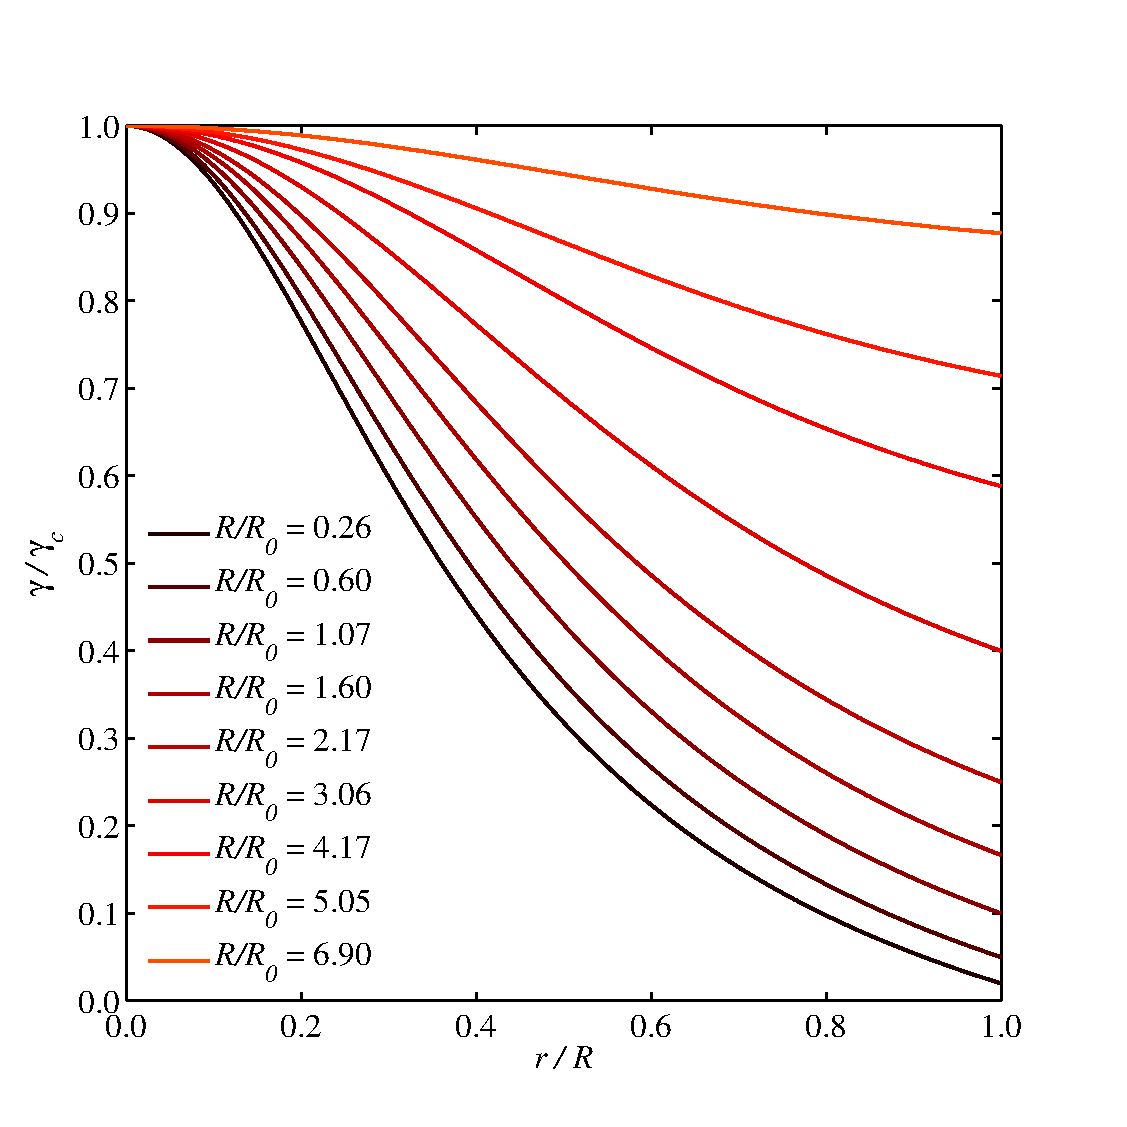
\includegraphics[width=0.46\textwidth]{gamma.eps} }
				\subfigure[Lorentz Factor at Center]{
					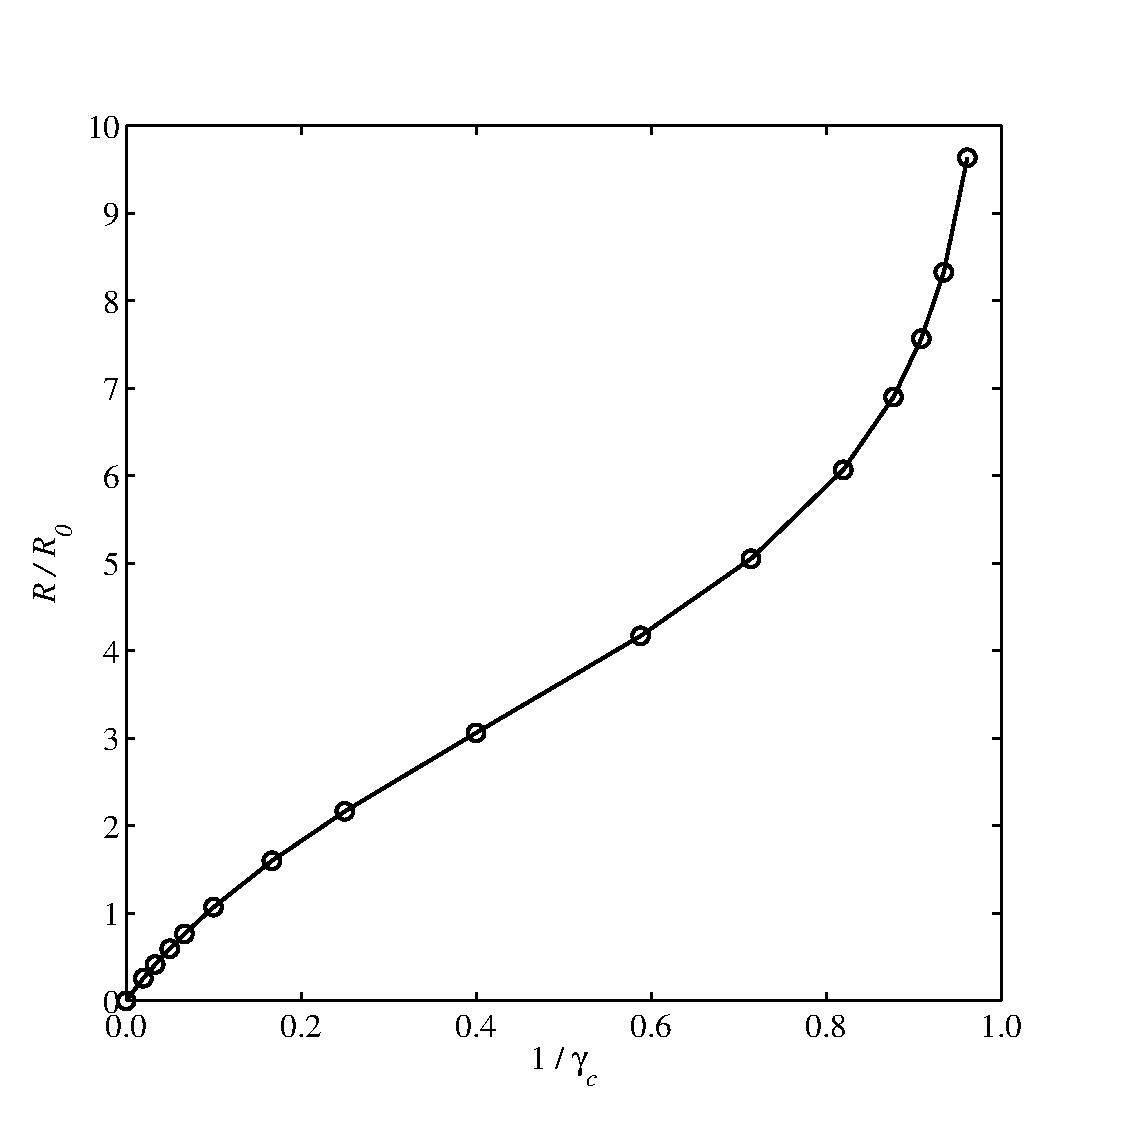
\includegraphics[width=0.46\textwidth]{gammar.eps} }
				\subfigure[Density Distribution]{
					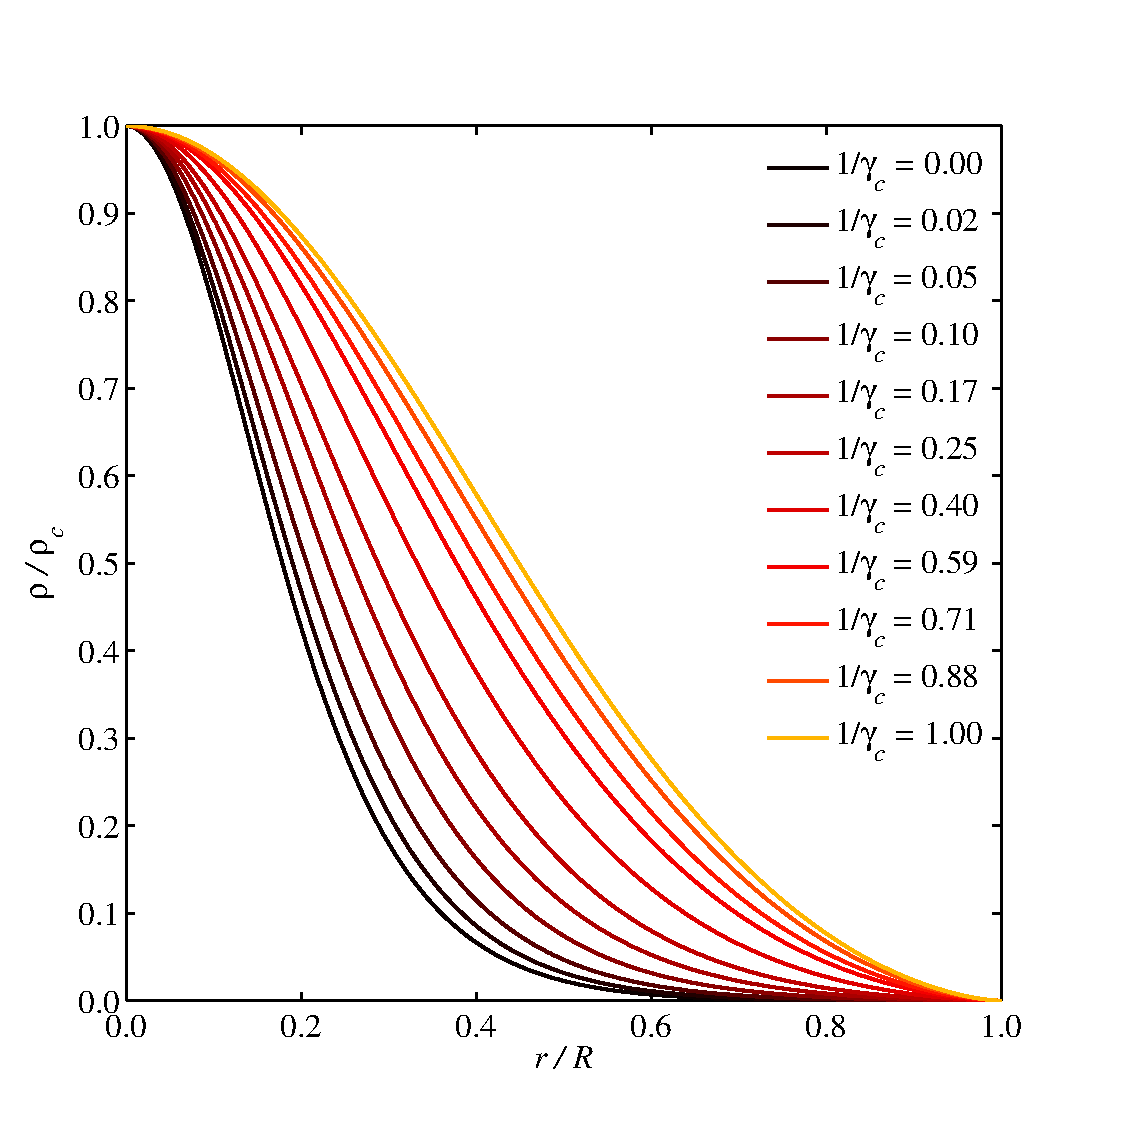
\includegraphics[width=0.46\textwidth]{rho2.eps} }
				\subfigure[Mass-Radius Relation]{
					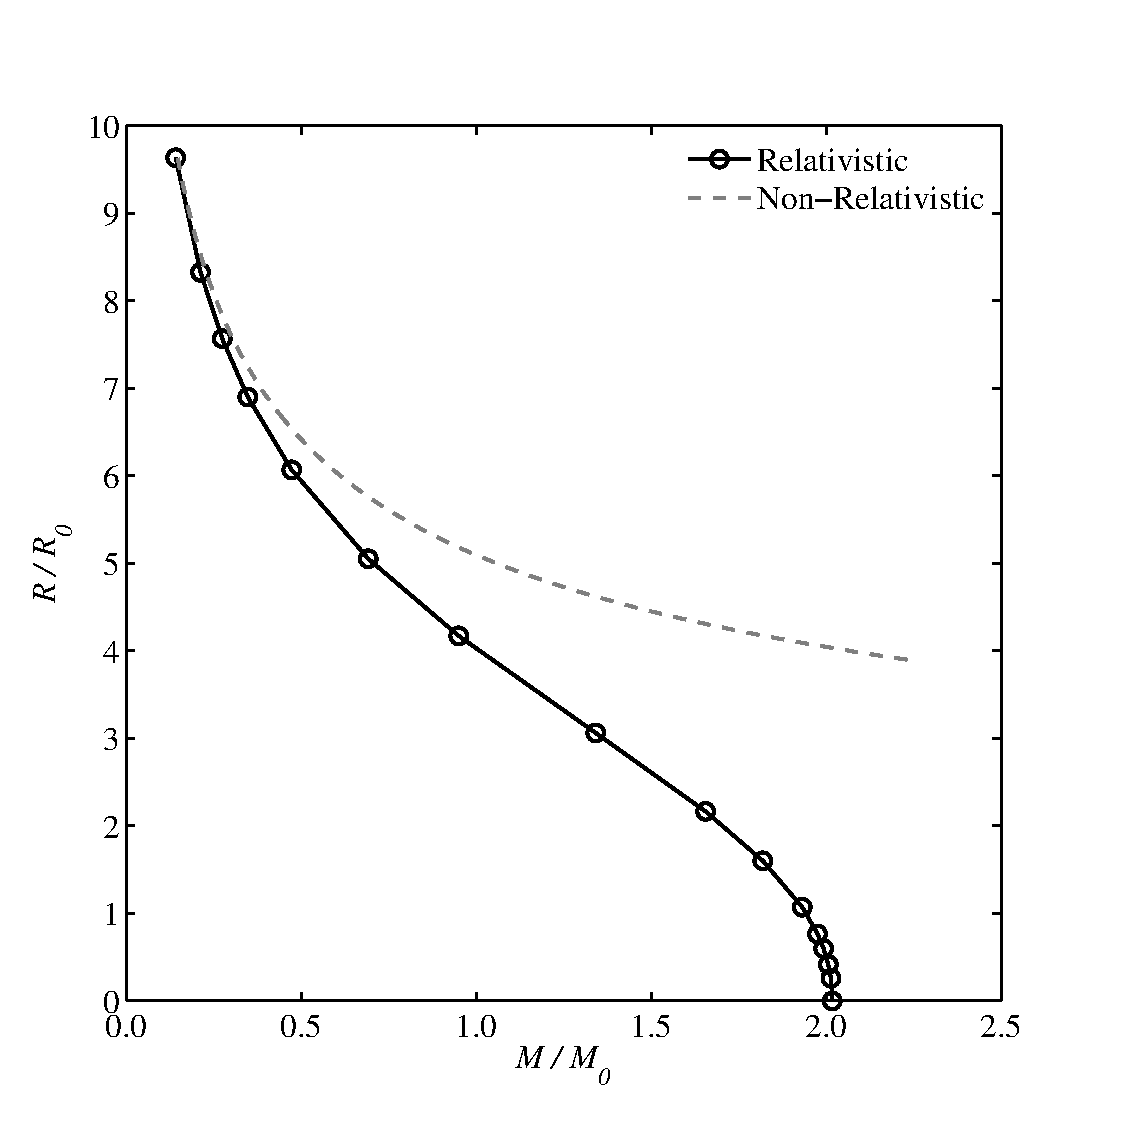
\includegraphics[width=0.46\textwidth]{mr1.eps} }
				\caption{The general solution and the derived results. In (b)(c)(d) former results at the non-relativstic limit and the ultra-relativistic limit are also added. }
				\label{fig:solution_general}
			\end{figure}
	
	
	\section{Conclusion}
		
		In this paper, we have discussed the equilibrium properties of non-rotating sphericla helium white dwarfs. Our key equation of equilibrium was derived on the distribution of electron chemical potential, and through the paper we solved it step by step. We noticed that the radius $R$ is variable in the equation, and different normalization should be applied to solve different cases. Solutions to the non-relativistic limit (for $R\rightarrow\infty$) and the ultra-relativistic limit (for $R\rightarrow0$) were obtained at first as they are relatively simple in treatment, and the exact value of Chandrasekhar limit could be obtained at this moment though its physical meaning was not fully revealed. For the general case, certain numerical techniques are required to solve the equation, and we found that the normalization proposed by Chandrasekhar was very helpful for its stability within the range of our interest. 
		
		The relativistic nature of the electrons is proved to be crucial. It arised from the beginning as we tried to estimate the electron degeneracy pressure of a typical white dwarf. Later inspection shows that the more compressed a white dwarf is, the more relativistic its electrons could be, and it reacts on the density distribution to concentrate more mass around the center. Back to the most concerned mass-radius relation, our result shows that the relativistc effect casts a significant boost on the drop of radius as mass increases, and the Chandrasekhar limit is not only the upper mass limit but also an unstable point where the star collapses drastically at $\mathdd R/\mathdd M\rightarrow\infty$. All these results are consistent with Chandrasekhar's original work.
		
		Further discussion may focus on the general relativistic correction to our model. Though we neglected the general relativistic effect estimting the escape velocity of a typical white dwarf, we cannot say for sure what would happen to those around the Chandrasekhar limit, extremely densed within an almost volumeless region. For such case, the Tolman-Oppenheimer-Volkoff (TOV) equation\cite{1939PhRv...55..374O} should be applied to the model. Other factors like rapid rotation, heavier elements, magnetic fields, etc, may also be taken into consideration.
	
	
	\section{Acknowledgement}
	This work is reformed from our course project of Mathmatical Physics II of 2017 spring, instructed by Prof. Chunyuan Gao, Peking University School of Physics. Other contributor to the original project includes Chenkai Mao, Ruixiao Yao, Youran Sun, and Zizhao Wang. We gratefully thank them for the foundation and improvement of this work.
	
	\bibliographystyle{unsrt}
	\bibliography{BibWhiteDwarf.bib}
%	\begin{thebibliography}{}
%		\bibitem{wiki} Wikipedia. White Dwarf, Sun
%		\bibitem{stat} Pathria. Statistical Mechanics
%		\bibitem{gr} Schultz. A First Course in General Relativity
%		\bibitem{climit} Chandrasekhar. The Highly Collapsed Configurations of a Stella Mass.
%	\end{thebibliography}

		

\end{document}